\section{Background and Motivating Example}

\subsection{Flaky tests and their categories}

A \emph{flaky test} passes and fails nondeterministically on the same code
revision and the same configuration. Following the taxonomy adopted by the
ReproFlake benchmark~\cite{zhang2026reproflake}, which refines the
well-established categories of~\cite{luo2014empirical}, we consider four
machine-reproducible categories:

\paragraph{Order-dependent (OD).}
The test fails only when another test runs before it in the same JVM, because
the earlier test (\emph{polluter}) mutates shared state (static fields,
singletons, external resources such as databases or files) that the later
test (\emph{victim}) assumes to be in its initial condition. OD failures
disappear when the test runs in isolation, which is precisely why developers
find them so confusing.

\paragraph{Time-dependent (TD).}
The test contains a race condition, a hard-coded deadline, a sleep, or a
timeout whose validity depends on machine speed, load, or clock behavior.
TD failures are aggravated by slow machines and parallel load.

\paragraph{Non-idempotent-outcome (NIO).}
The test mutates state that it does not restore, so that a \emph{second}
execution of the same test in the same JVM observes polluted state and fails
— even though every isolated run passes. NIO tests are order-independent but
self-polluting.

\paragraph{Implementation-dependent (ID).}
The test relies on nondeterministic JVM behavior — hash iteration order,
reflection order, random seeds, floating-point environmental factors — so its
assertions are only accidentally true for some implementations.

\subsection{Motivating example}

\begin{figure}[t]
\centering
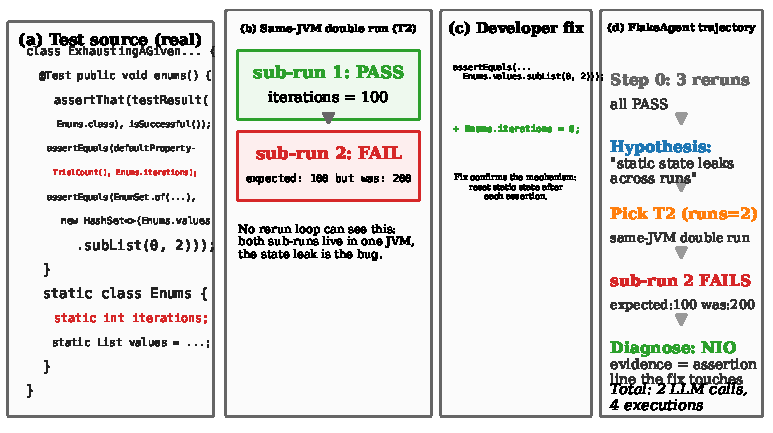
\includegraphics[width=0.9\columnwidth]{figures/motivating_example.pdf}
\caption{The \texttt{enums} test from Apache QuickCheck (ID
\texttt{quickcheck485} in our benchmark) as a motivating example.
(a) The test launches a nested property-based test class inside itself and
asserts on the \emph{static} accumulators \texttt{Enums.iterations} and
\texttt{Enums.values}. (b) Running \texttt{enums} twice in the same JVM:
the first run passes; the second fails with
\texttt{expected: 100 but was: 200}, because the static accumulators were not
reset. This is a textbook NIO failure. (c) The developer fix — resetting the
static state after each assertion — which we use as ground truth for
evidence evaluation. (d) FlakeAgent's cold-start trajectory: three baseline
reruns all pass; the agent hypothesizes self-pollution and selects the
same-JVM double-run strategy; the second sub-run fails; the agent diagnoses
NIO and cites the exact assertion line the developer fixed.}
\label{fig:motivating}
\end{figure}

Figure~\ref{fig:motivating} shows a real motivating example: the
\texttt{enums} test in \texttt{junit-quickcheck} runs a nested test class
inside itself and asserts on static accumulators, so it passes in isolation
but fails deterministically on a \emph{second execution in the same JVM}. This
example demands three things of any tool that wants to help: (i) the failure
never appears in a normal rerun, so rerun- or log-based tools are blind to
it; (ii) the trigger is a deliberate execution scheme (same-JVM double run);
and (iii) the diagnosis is grounded in the failing assertion and surrounding
code. FlakeAgent is designed around exactly this structure
(Section~\ref{sec:approach}).

\subsection{The ReproFlake benchmark}

ReproFlake~\cite{zhang2026reproflake} is a recent dataset of 1{,}115
machine-reproducible flaky tests from 63 JIRA issues and 1{,}052 commits of
the iDoFT dataset~\cite{parry2022survey}, spanning 819 implementation-dependent,
126 order-dependent, 125 non-idempotent, 36 time-dependent, and 9 uncategorized
tests. For each test it ships the project snapshot at the flaky commit
(\texttt{Flaky/}), the developer fix as a patch (\texttt{Fixed.patch}), a
Maven dependency cache (\texttt{Flakym2/}), and — crucially for evaluation —
the \emph{official reproduction mechanism} of the category that was used to
machine-confirm the flakiness: manual sleep injection at a timing-sensitive
line for TD (shipped as a \texttt{FlakyCodeChange.patch} reproduction patch),
polluter--victim ordered runs for OD, the iDFlakies same-JVM double-run plugin
for NIO, and the NonDex nondeterminism injector for ID. We use these mechanisms (i) as a
validation gate for our subset and (ii) as the \emph{warm-start} configuration
in one ablation. The developer fix patch serves as ground truth for our
diagnosis evaluation: we check whether the evidence lines the agent cites
were touched by the fix commit.
